\section{AirBnb Price Estimator App}

\subsection{Introduction}
\textbf{AirBnB Price Estimator} is a real estate cost estimation application in which the \textit{Users} insert some informations related to the B\&B they want to compute the price.

\subsection{Use Cases List}
There is no need for registration, every user can operate with the \textit{applicative} as they open it. The \textbf{use cases} are:

\begin{itemize}
	\item Select the classifier to use
		\subitem - \textit{Random Forest}
		\subitem - \textit{M5Rules}
	\item Insert values for requested B\&B related characteristics
	\item Compute the price using the algorithm previously selected
\end{itemize}

\subsection{Application Guide}
When the application is launched a window is opened telling the \textit{User} to choose between the two classifier previously discussed. The \textit{User} cannot undo the choose, if he/she clicks the incorrect classifier he/she has to reopen the application.

\begin{figure}[H]
	\centering
	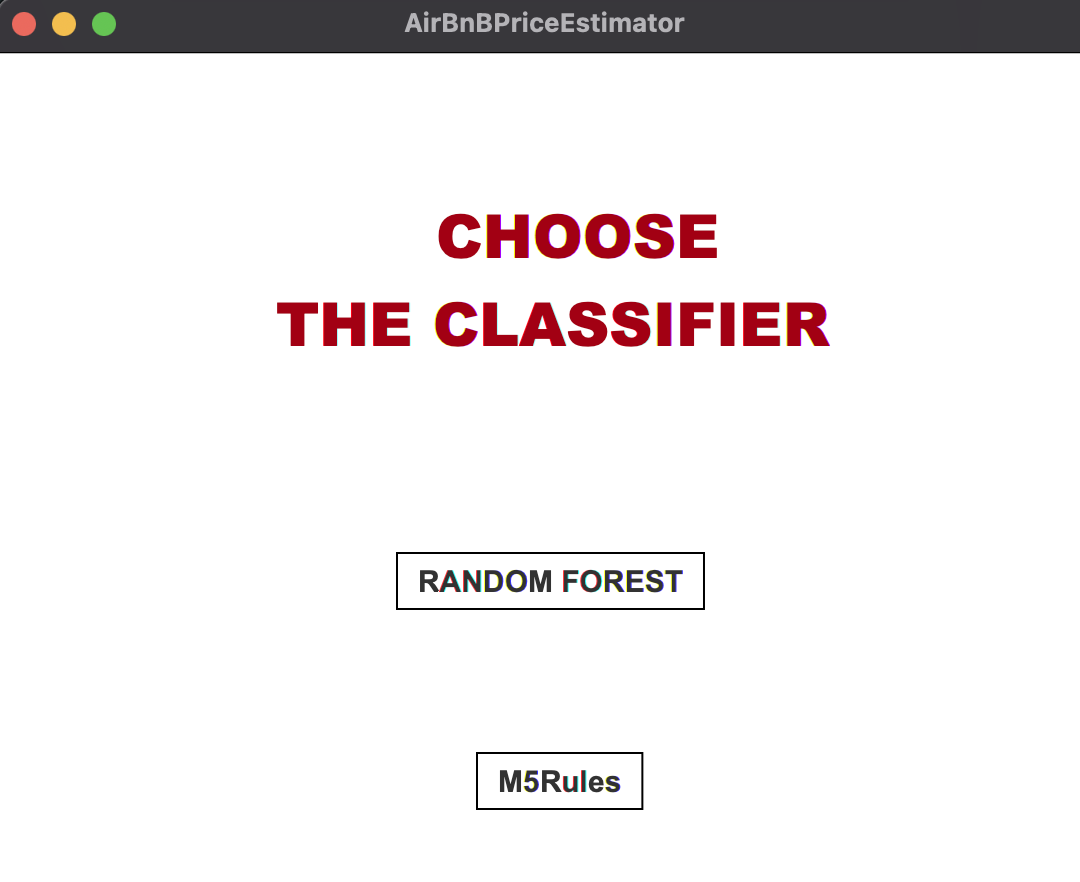
\includegraphics[width=0.6\textwidth]{img/app.png}  
\end{figure}

Selected the classifier, a new scene is loaded. This scene displays some \textit{TextField}s and \textit{RadioButton}s, those refer to a subset of the overall features in out dataset that is evaluated in the \textit{Attribute Selection} process we talked about in chapter 3.3.

\begin{figure}[H]
	\centering
	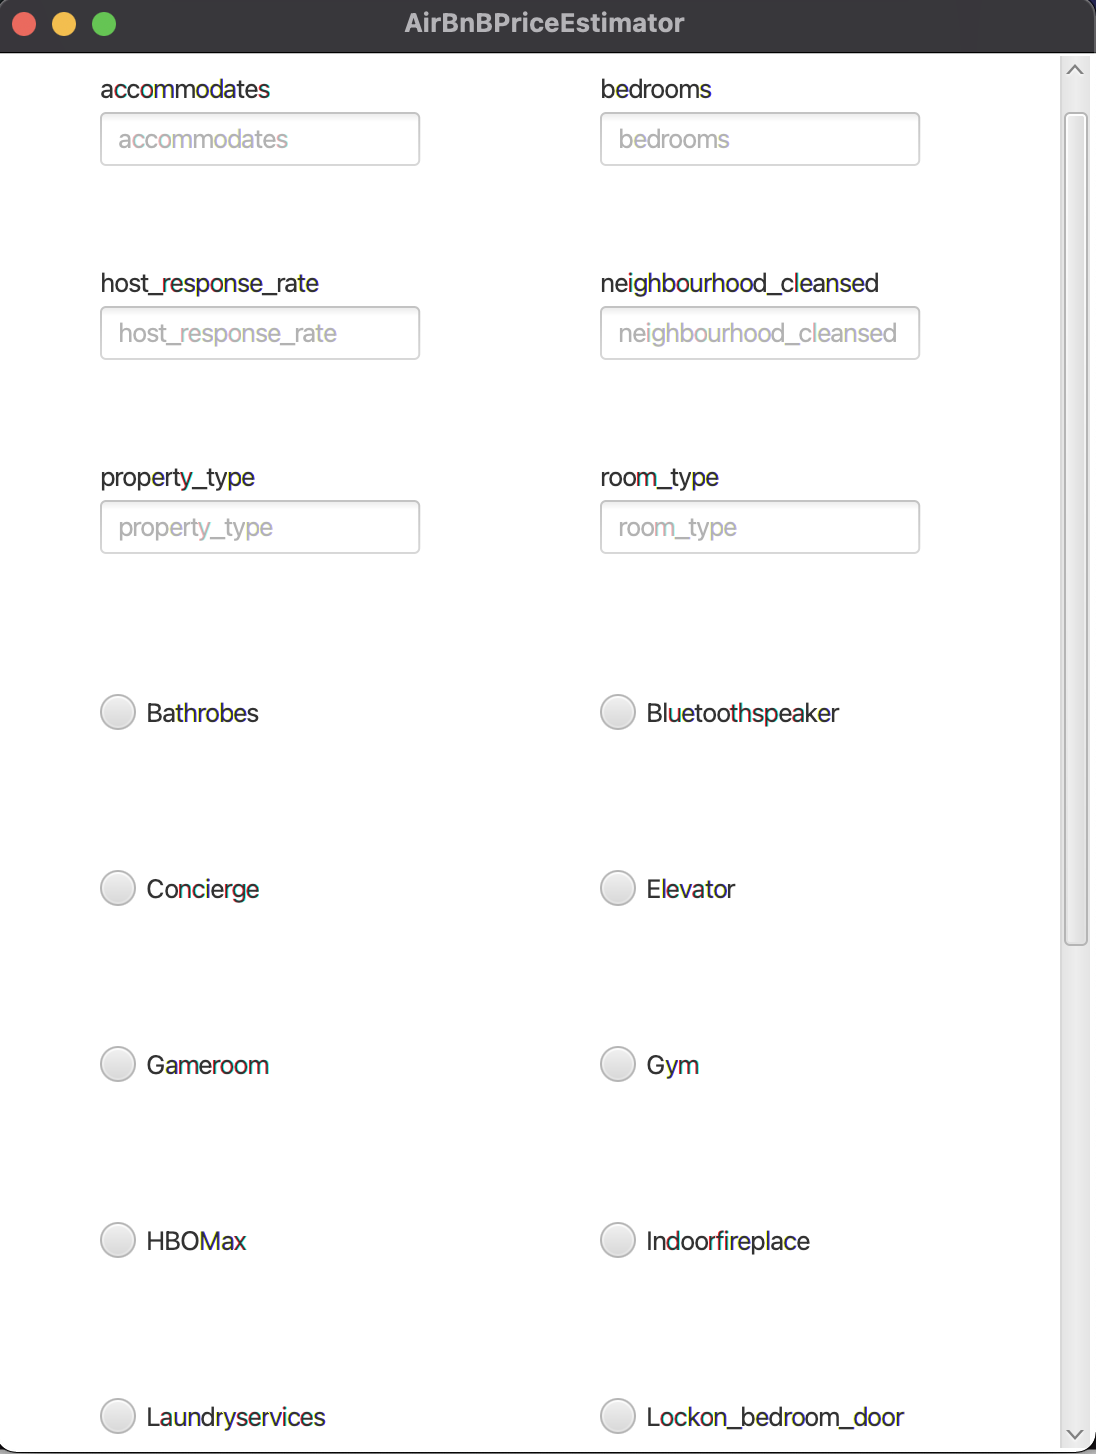
\includegraphics[width=0.6\textwidth]{img/mainApp.png}  
\end{figure}

If a \textit{RadioButton} is not selected the system will understand that as the absence of the particular amenity the \textit{RadioButton} refers to.

After the \textit{User} imputes all the values a \textit{Button} saying \textit{"PREDICT PRICE"} is located at the button of the window (scroll down if you don't see it). After clicked on it,  a label displaying the predicted price is shown below the \textit{Button}.


\begin{figure}[H]
	\centering
	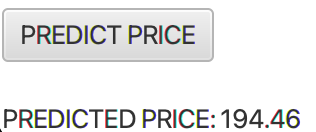
\includegraphics[width=0.3\textwidth]{img/pricePredicted.png}  
\end{figure}